\chapter{Generowanie grafów}
\textit{Autorzy rozdziału: Krzysztof Karpusiewicz, Mateusz Kołakowski}
\vspace{0.5cm}\newline
\section{Rozszerzanie grafu}
\textit{Autor podrozdziału: Krzysztof Karpusiewicz}
\vspace{0.5cm}\newline
%Do przeprowadzenia poprawnego rozumowania na grafach, wymagane jest wpierw pozyskanie zbioru grafów. Operację tę nazywamy generowaniem grafów, i rozpoczyna się ją od rozszerzania grafów. 
Aby przeprowadzać operacje na wielu grafach, najpierw należy je wygenerować, metoda która służy do generowania grafów nazywa się rozszerzaniem grafów. 
\begin{definition} Rozszerzeniem grafu nazywamy przekształcenie grafu $G$ w graf $G'$ poprzez dodanie do $G$ wierzchołka $v$ i dowolnego podzbioru możliwych krawędzi pomiędzy $v$ a $V(G)$.
\end{definition}
Możliwych rozszerzeń grafu o $n$ wierzchołkach jest $2^n$. Kompletnym rozszerzeniem nazywamy zbiór grafów uzyskany przez wykonanie każdego możliwego rozszerzenia.

Najprostszym przykładem rozszerzenia grafu jest rozszerzanie grafu jednowierzchołkowego, pokazanego na rys. \ref{grafjednowierzcholkowy}.
\begin{figure}[H]
  \centering
  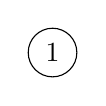
\begin{tikzpicture}[node distance={15mm}, main/.style = {draw, circle}] 
    \node[main] (1) {$1$};
   \end{tikzpicture}
   \caption{Graf jednowierzchołkowy}
   \label{grafjednowierzcholkowy}
\end{figure}


Podczas rozszerzania powyższego grafu istnieją dwie możliwości na sposób dodania krawędzi pomiędzy Grafem $G$ a nowym wierzchołkiem. W celu wygenerowania wszystkich grafów dwuwierzchołkowych należy przeprowadzić rozszerzenia na wszystkie (dwa) możliwe sposoby jak na rysunku \ref{rozszerzeniedwuwierzcholkowe}.
\begin{figure}[H]
  
  \centering
  \subfloat[]{
  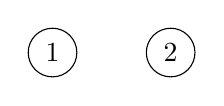
\begin{tikzpicture}[node distance={15mm}, main/.style = {draw, circle}] 
    \node[main] (2) {$1$};
    \node[main] (3) [right of=2] {$2$};
   \end{tikzpicture}
   }
   \hspace{15mm}
   \subfloat[]{
   \begin{tikzpicture}[node distance={15mm}, main/.style = {draw, circle}] 
    \node[main] (1)  {$1$};
    \node[main] (2) [right of=2] {$2$};
    \draw (1) -- (2);
   \end{tikzpicture}  
   }

   \caption{Oba możliwe rozszerzenia grafu jednowierzchołkowego}
   \label{rozszerzeniedwuwierzcholkowe}
\end{figure}

W podobny sposób można uzyskać kompletny zbiór grafów o dowolnej liczbie wierzchołków. Wystarczy jedynie rekurencyjnie rozszerzać zbiór grafów, zaczynając od jednego wierzchołka i kończąc, gdy nasz zbiór zawiera grafy o wymaganym rzędzie. Przez rozszerzenie zbioru grafów mamy na myśli rozszerzenie każdego z grafów ze zbioru na wszystkie możliwe sposoby. 

Takie podejście prowadzi co prawda  do uzyskania każdego możliwego grafu, jest jednak zatrważająco nieefektywne. Jest tak, ponieważ takie generowanie generuje zbiory grafów zawierające pełne grupy grafów izomorficznych, które, ze względu na naturę problemu poruszanego w tej pracy, nie wnoszą więcej informacji, niż jeden jej przedstawiciel. Dzieje się tak głównie ze względu na fakt, że izomorfizm nie zmienia największego stopnia kliki, ani zbioru niezależnego w grafie.

W celu zobrazowania problemu przeprowadźmy dalsze rozszerzenie dwuwierzchołkowego grafu pełnego z rysunku \ref{rozszerzeniedwuwierzcholkowe}. Określmy ten graf jako graf $G$. Rozszerzenie grafu dwuwierzchołkowego w sposób kompletny prowadzi do uzyskania 4 grafów, pokazanych na rysunku \ref{rozszerzenietrzywierzcholki}.


\begin{figure}[H]
		\centering
		\subfloat[]{
  		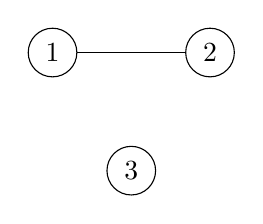
\begin{tikzpicture}[node distance={15mm}, main/.style = {draw, circle}] 
   			\node[main] (0) at (0,1.5) {$1$};
   			\node[main] (1) at (2,1.5)  {$2$};
   			\node[main] (2) at (1,0)  {$3$};
   			
   			\draw (0) -- (1);
   		\end{tikzpicture}
   		}
   		\hspace{5mm}
   		\subfloat[]{
		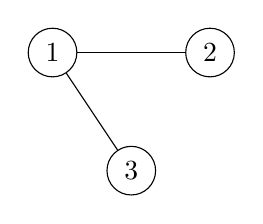
\begin{tikzpicture}[node distance={15mm}, main/.style = {draw, circle}] 	
			\node[main] (3) at (3,1.5) {$1$};
   			\node[main] (4) at (5,1.5)  {$2$};
   			\node[main] (5) at (4,0)  {$3$};
   			
   			\draw (3) -- (4);
   			\draw (3) -- (5);
   		\end{tikzpicture}
   		}
   		\hspace{5mm}
   		\subfloat[]{
		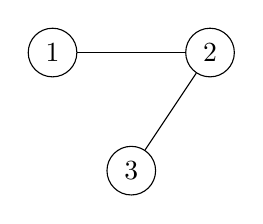
\begin{tikzpicture}[node distance={15mm}, main/.style = {draw, circle}] 	
			\node[main] (6) at (6,1.5) {$1$};
   			\node[main] (7) at (8,1.5)  {$2$};
   			\node[main] (8) at (7,0)  {$3$};
   			
   			\draw (6) -- (7);
   			\draw (7) -- (8);
   		\end{tikzpicture}
   		}
   		\hspace{5mm}
   		\subfloat[]{
		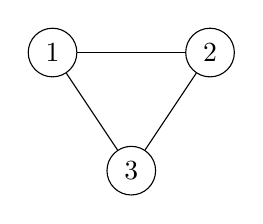
\begin{tikzpicture}[node distance={15mm}, main/.style = {draw, circle}] 	
			\node[main] (9) at (9,1.5) {$1$};
   			\node[main] (10) at (11,1.5)  {$2$};
   			\node[main] (11) at (10,0)  {$3$};
			
			\draw (9) -- (10);
			\draw (9) -- (11);
			\draw (10) -- (11);
			
   		\end{tikzpicture}
   		}
   		\hspace{5mm}
   		\caption{Możliwe rozszerzenia grafu $G$ opisane dalej jako $G'_1$ do $G'_4$}
   		\label{rozszerzenietrzywierzcholki}
\end{figure}

Warto zauważyć, że powstały zbiór 4 grafów zawiera dwa grafy izomorficzne, $G'_2$ i $G'_3$. Można więc powiedzieć, że zbiór $\mathcal{G'}$ zawiera trzy zbiory grafów izomorficznych. W przypadku grafów trójwierzchołkowych wygenerowanych przez rozszerzenie grafów na rysunku \ref{rozszerzeniedwuwierzcholkowe}, uzyskamy 8 grafów, ale jedynie 4 grupy izomorficzne. Trywialnie więc zauważyć, że jeżeli do zbioru $\mathcal{G'}$ dodamy również rozszerzenia drugiego grafu z \ref{rozszerzeniedwuwierzcholkowe} przybędzie tylko jeden unikatowy graf.

 Wyeliminowanie nadmiarowych grafów izomorficznych ze zbioru wynikowego jest wysoko pożądane w celu zwiększenia wydajności generacji zarówno pod względem czasowym jak i pamięciowym. Żeby zobrazować wagę takiej optymalizacji wystarczy podać kilka pierwszych wartości dla ilości grafów wygenerowanych naiwną metodą rozszerzania w porównaniu do ilości grafów nieizomorficznych.
 \begin{table}[H]
 \begin{center}
 \begin{tabular}{|c c c|} 
 \hline
 Rząd grafów & Ilość rozszerzeń\cite{OEIS2} & Ilość grafów nieizomorficznych\cite{OEIS}  \\ 
 \hline\hline
 1 & 1 & 1  \\ 
 \hline
 2 & 2 & 2  \\
 \hline
 3 & 8 & 4  \\
 \hline
 4 & 64 & 11  \\
 \hline
 5 & 1024 & 34  \\
 \hline
 6 & 32768 & 156  \\
 \hline
 7 & 2097152 & 1044  \\
 \hline
 8 & 268435456 & 12346  \\
 \hline
\end{tabular}
\end{center}
 \caption{Tabela porównująca ilość możliwych rozszerzeń i ilość grafów nieizomorficznych w przypadku tworzenia kompletnego zbioru grafów określonego rzędu}
 \end{table}

\section{Generowanie grafów nieizomorficznych}
\textit{Autor podrozdziału: Mateusz Kołakowski}
\vspace{0.5cm}\newline
Użytecznym jest fakt, że na dowolnym etapie generacji zbiór grafów izomorficznych w zbiorze do rozszerzenia można bezproblemowo zredukować do tylko jednego z jego przedstawicieli. Jest tak ze względu na poniższe twierdzenie.
\begin{theorem}
Jeżeli rozszerzamy izomorficzne grafy $G$ oraz $H$ do zbiorów $\mathcal{G'}$ oraz $\mathcal{H'}$, to dla dowolnego elementu zbioru $\mathcal{G'}$ istnieje izomorfizm do elementu zbioru $\mathcal{H'}$
\end{theorem}


Dzięki powyższemu twierdzeniu, jeżeli na każdej iteracji generacji grafów będziemy usuwać nadmiarowe grafy izomorficzne to wynikowy zbiór grafów nie będzie zawierał  grafów rozszerzonych z grafów już izomorficznych, ale nie straci żadnych istotnych dla nas grafów. Dzięki temu, pozostają dwie możliwości powstania zbiorów grafów izomorficznych do zredukowania: grafy izomorficzne powstałe z rozszerzania różnych grafów, oraz grafy izomorficzne powstałe z rozszerzania tego samego grafu. Obie te możliwości można eliminować, nie porównując grafów w stylu "każdy z każdym". Podejście takie jest wysoko pożądane, jako że znajdywanie izomorfizmów w zbiorze grafów to problem nietrywialny, który mógłby znacznie spowolnić działanie generacji. Aby zobrazować metody eliminowania, na rysunku \ref{rozszerzenieIzomorfizm1} jest pokazany zbiór grafów izomorficznych wynikających z rozszerzenia grafów dwuwierzchołkowych. 

\begin{figure}[H]
	\hfill
	\subfloat[]{
	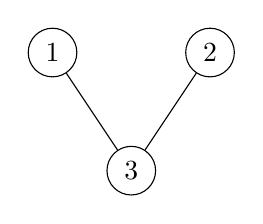
\begin{tikzpicture}[node distance={15mm}, main/.style = {draw, circle}] 
   		\node[main] (0) at (0,1.5) {$1$};
   		\node[main] (1) at (2,1.5)  {$2$};
   		\node[main] (2) at (1,0)  {$3$};
    	\draw (0) -- (2);
		\draw (1) -- (2);
	\end{tikzpicture}
	}
	\hfill
	\subfloat[]{
	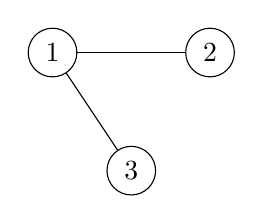
\begin{tikzpicture}[node distance={15mm}, main/.style = {draw, circle}] 
   		\node[main] (0) at (0,1.5) {$1$};
   		\node[main] (1) at (2,1.5)  {$2$};
   		\node[main] (2) at (1,0)  {$3$};
    	\draw (0) -- (2);
		\draw (0) -- (1);
	\end{tikzpicture}
	}
	\hfill
	\subfloat[]{
	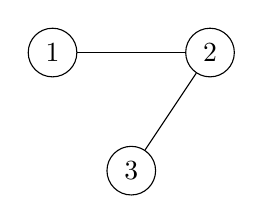
\begin{tikzpicture}[node distance={15mm}, main/.style = {draw, circle}] 
   		\node[main] (0) at (0,1.5) {$1$};
   		\node[main] (1) at (2,1.5)  {$2$};
   		\node[main] (2) at (1,0)  {$3$};
    	\draw (1) -- (2);
		\draw (1) -- (0);
	\end{tikzpicture}
	}
	\hfill
	\hfill
	\caption{Zbiór grafów izomorficznych powstający z rozszerzania grafów dwuwierzchołkowych}
	\label{rozszerzenieIzomorfizm1}
\end{figure} 
Powyższe grafy będą opisywane jako $G_1$, $G_2$ i $G_3$. Aby eliminować izomorfizmy powstałe z rozszerzania różnych grafów każdy z grafów $G'$ należy sprowadzić do formy kanonicznej a następnie wyznaczyć istniejące w nim orbity. Przykładowym przekształceniem grafu $G_3$ do formy kanonicznej jest 
$$ \{1,2,3\} \to \{2,1,3\} $$
Efektem takiego przekształcenia dla grafów $G_1$ i $G_2$ są grafy przedstawiony na rysunku \ref{g2canon}

\begin{figure}[H]
	\centering
	\hfill
	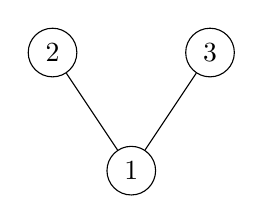
\begin{tikzpicture}[node distance={15mm}, main/.style = {draw, circle}] 
   		\node[main] (2) at (0,1.5) {$2$};
   		\node[main] (0) at (2,1.5)  {$3$};
   		\node[main] (1) at (1,0)  {$1$};
    	\draw (1) -- (2);
		\draw (0) -- (1);
	\end{tikzpicture}
	\hfill
	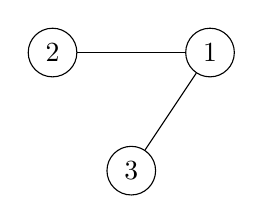
\begin{tikzpicture}[node distance={15mm}, main/.style = {draw, circle}] 
   		\node[main] (2) at (0,1.5) {$2$};
   		\node[main] (0) at (2,1.5)  {$1$};
   		\node[main] (1) at (1,0)  {$3$};
    	\draw (0) -- (2);
		\draw (0) -- (1);
	\end{tikzpicture}
	\hfill
	\hfill
	\caption{Grafy $G_2$ i $G_3$ w formie kanonicznej}
	\label{g2canon}
\end{figure} 

Orbitami tych grafów są zbiory \{1\} oraz \{2,3\}. Większość grafów można uzyskać przez rozszerzenie kilku różnych grafów, ale nowo dodany wierzchołek, czyli ten o największym numerze przed przekształceniem grafu na formę kanoniczną, znajdzie się w jakiejś orbicie $o$ tylko dla rozszerzeń z jednego grafu $G$ z nieizomorficznego zbioru $\mathcal{G}$. Wystarczy więc jedynie sprawić, że grafy $G'$ zostaną odrzucone, jeżeli ich najnowszy wierzchołek nie znajdzie się w określonej orbicie. Należy też sprawić, aby ta sama orbita została wybrana jako kryterium dla wszystkich grafów $G`$, co sprawia się przez przekształcenie na formę kanoniczną. Takie odrzucanie pozwala wyeliminować wszystkie grafy izomorficzne powstałe przez rozszerzanie różnych grafów. 
Kontynuując przykład z rysunku \ref{g2canon}, nowy wierzchołek tego grafu znajduje się w orbicie pierwszej dla $G_1$, ale w orbicie drugiej dla $G_2$. Oznacza to, że graf $G_2$ byłby odrzucony bez potrzeby porównywania go do grafu $G_1$.

Drugim przykładem grafów izomorficznych do odrzucenia są grafy powstałe przez rozszerzanie jednego grafu. Przykład takich grafów, na rysunku \ref{rozszerzenieIzomorfizm1}, to grafy $G_2$ oraz $G_3$. Takie grafy eliminowane są przy użyciu grup automorfizmów grafu $G$. Łącząc nowy wierzchołek z $n$ elementami orbity generowanej przez grupy automorfizmów, możemy dokonać pewnych odrzuceń. Zachowujemy dany graf tylko jeżeli nowy wierzchołek został połączony z $n$ elementami orbity, którym sprowadzenie do formy kanonicznej przyporządkowało najniższe numery.


\section{Generowanie grafów Ramesyowskich}
\textit{Autorzy podrozdziału: Krzysztof Karpusiewicz, Mateusz Kołakowski}
\vspace{0.5cm}\newline
Generowanie grafów nieizomorficznych jest wciąż zbyt wymagające dla naszych potrzeb. Ilość grafów nieizomorficznych poszczególnych rzędów rośnie wykładniczo, i dla grafów rzędu 17, największego generowanego przez rozszerzanie w tej pracy, byłoby ich ponad $2 \cdot 10^{26}$\cite{OEIS}. Jasnym więc jest, że ilość grafów generowanych na poszczególnych etapach rozszerzania należy bardziej ograniczyć. Z pomocą przychodzi następujące twierdzenie: 


\begin{theorem}
	Dla dowolnego grafu $G$ posiadającego klikę $K_i$ każdy graf $H$, który powstaje przez dowolną sekwencję rozszerzeń grafu $G$, zawiera klikę $K_j$ gdzie $j \geq i$.
\label{tw5}
\end{theorem}


Powyższe twierdzenie wynika z  następującego rozumowania:

 Gdy graf $G$ rozszerzymy do grafu $G'$, to graf $G$ jest podgrafem grafu $G'$. Dzieje się tak, ponieważ rozszerzanie nie modyfikuje krawędzi w oryginalnym grafie, a jedynie dodaje krawędzie do nowego wierzchołka. Przy pomocy indukcji matematycznej można więc powiedzieć, że dowolny graf $H$, który powstaje poprzez wielokrotne rozszerzanie grafu $G$ musi zawierać graf $G$ jako swój podgraf. Z tego powodu, graf $H$ musi również zawierać klikę z oryginalnego grafu $G$, oraz może posiadać klikę większą powstałą w wyniku rozszerzania. Przykład zachowania oryginalnego grafu podczas rozszerzania jest pokazany na rysunku \ref{rozszerzeniekliki}

\begin{figure}[H]
\subfloat[]{
  		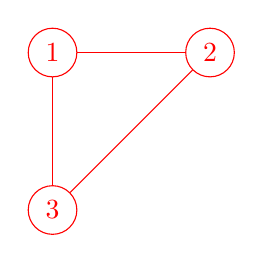
\begin{tikzpicture}[node distance={15mm}, main/.style = {draw, circle}] 
   			\node[main][red] (0) at (0,2) {$1$};
   			\node[main][red] (1) at (2,2)  {$2$};
   			\node[main][red] (2) at (0,0)  {$3$};
			\draw[red] (0) -- (1);
			\draw[red] (0) -- (2);,
			\draw[red] (1) -- (2);
		\end{tikzpicture}
		}	
		\hspace{15mm}
		\subfloat[]{
		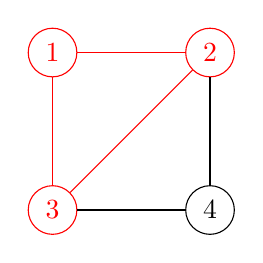
\begin{tikzpicture}[node distance={15mm}, main/.style = {draw, circle}] 	
			\node[main][red] (3) at (4,2) {$1$};
   			\node[main][red] (4) at (6,2)  {$2$};
   			\node[main][red] (5) at (4,0)  {$3$};
   			\node[main] (6) at (6,0)  {$4$};
			\draw[red] (3) -- (4);
			\draw[red] (3) -- (5);,
			\draw[red] (4) -- (5);
			\draw (6) -- (5);
			\draw (6) -- (4);
		\end{tikzpicture}
		}
		\hspace{15mm}
		\subfloat[]{
		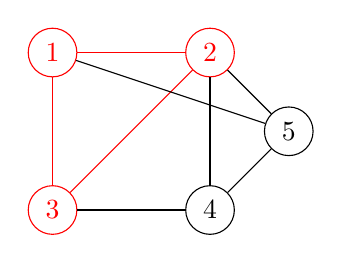
\begin{tikzpicture}[node distance={15mm}, main/.style = {draw, circle}]	
			\node[main][red] (7) at (8,2) {$1$};
   			\node[main][red] (8) at (10,2)  {$2$};
   			\node[main][red] (9) at (8,0)  {$3$};
   			\node[main] (10) at (10,0)  {$4$};
   			\node[main] (11) at (11,1)  {$5$};
			\draw[red] (7) -- (8);
			\draw[red] (7) -- (9);,
			\draw[red] (8) -- (9);
			\draw (10) -- (8);
			\draw (10) -- (9);
			\draw (11) -- (10);
			\draw (11) -- (7);
			\draw (11) -- (8);
			
			
   		\end{tikzpicture}
   		}
		\linebreak
		\subfloat[]{
  		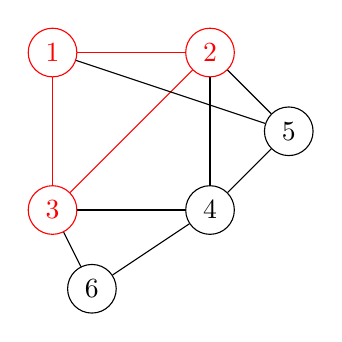
\begin{tikzpicture}[node distance={15mm}, main/.style = {draw, circle}] 
			\node[main][red] (7) at (0,2) {$1$};
   			\node[main][red] (8) at (2,2)  {$2$};
   			\node[main][red] (9) at (0,0)  {$3$};
   			\node[main] (10) at (2,0)  {$4$};
   			\node[main] (11) at (3,1)  {$5$};
   			\node[main] (12) at (0.5,-1)  {$6$};
			\draw[red] (7) -- (8);
			\draw[red] (7) -- (9);,
			\draw[red] (8) -- (9);
			\draw (10) -- (8);
			\draw (10) -- (9);
			\draw (11) -- (10);
			\draw (11) -- (7);
			\draw (11) -- (8);
			\draw (12) -- (9);
			\draw (12) -- (10);
			
		\end{tikzpicture}
		}
		\hspace{15mm}
		\subfloat[]{
		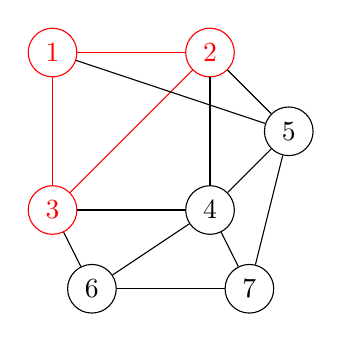
\begin{tikzpicture}[node distance={15mm}, main/.style = {draw, circle}] 	
			\node[main][red] (1) at (4,2) {$1$};
   			\node[main][red] (2) at (6,2)  {$2$};
   			\node[main][red] (3) at (4,0)  {$3$};
   			\node[main] (4) at (6,0)  {$4$};
			\node[main] (5) at (7,1)  {$5$};
   			\node[main] (6) at (4.5,-1)  {$6$};
			\node[main] (Z) at (6.5,-1)  {$7$};
			\draw[red] (1) -- (2);
			\draw[red] (1) -- (3);,
			\draw[red] (2) -- (3);
			\draw (4) -- (2);
			\draw (4) -- (3);
			\draw (4) -- (5);
			\draw (5) -- (1);
			\draw (5) -- (2);
			\draw (6) -- (3);
			\draw (6) -- (4);
			\draw (Z) -- (6);
			\draw (Z) -- (4);
			\draw (Z) -- (5);
		
		\end{tikzpicture}
		}
		\hspace{15mm}
		\subfloat[]{
		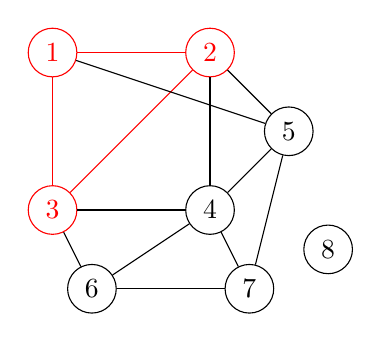
\begin{tikzpicture}[node distance={15mm}, main/.style = {draw, circle}] 	
			\node[main][red] (7) at (8,2) {$1$};
   			\node[main][red] (8) at (10,2)  {$2$};
   			\node[main][red] (9) at (8,0)  {$3$};
   			\node[main] (10) at (10,0)  {$4$};
   			\node[main] (11) at (11,1)  {$5$};
   			\node[main] (12) at (8.5,-1)  {$6$};
			\node[main] (13) at (10.5,-1)  {$7$};
			\node[main] (14) at (11.5,-0.5)  {$8$};
			\draw[red] (7) -- (8);
			\draw[red] (7) -- (9);,
			\draw[red] (8) -- (9);
			\draw (10) -- (8);
			\draw (10) -- (9);
			\draw (11) -- (10);
			\draw (11) -- (7);
			\draw (11) -- (8);
			\draw (12) -- (9);
			\draw (12) -- (10);
			\draw (12) -- (13);
			\draw (11) -- (13);
			\draw (10) -- (13);

   		\end{tikzpicture}
   		}
   		\caption{Kolejne rozszerzenia grafu. (graf początkowy zaznaczony kolorem czerwonym)}
   		\label{rozszerzeniekliki}
\end{figure}
Identyczne rozumowanie można przeprowadzić dla zbiorów niezależnych w oryginalnym grafie, prowadząc do analogicznego twierdzenia dotyczącego zbiorów niezależnych.
\begin{theorem}
Dla dowolnego grafu $G$ posiadającego zbiór niezależny $N_i$ każdy graf $H$, który powstaje przez dowolną sekwencję rozszerzeń grafu $G$, zawiera zbiór niezależny $N_j$ gdzie $j \geq i$.
\label{tw6}
\end{theorem}
Twierdzenia te prowadzą do wniosku podobnego do tego o eliminacji grafów izomorficznych, gdzie jeżeli na każdym etapie algorytmu wyeliminujemy grafy łamiące ograniczenia dotyczące kliki oraz zbioru niezależnego, zapewni to, że każdy graf na podstawie którego będziemy generować kolejne grafy nie łamie ograniczeń. Grafy łamiące ograniczenia możemy eliminować, ponieważ na podstawie twierdzeń \ref{tw6} i \ref{tw5} w wyniku ich rozszerzenia powstają jedynie grafy które i tak zostałyby odrzucone. Dzięki temu można znacznie ograniczyć ilość grafów tworzonych na późniejszych etapach generacji. 
Omówione ograniczenia prowadzą do powstania algorytmu generacji grafów w następującej formie:

\begin{algorithm}[H]
  \caption{Generowanie grafów ramseyowskich o podanym stopniu}
  \begin{algorithmic}
  \REQUIRE $n > 0 \land r>1 \land b>1$
  \STATE $i \gets 1$
  \STATE grafy[] $\gets$ graf jednowierzchołkowy 
  \WHILE{$i < n$}
    \STATE rozszerz(grafy)
    \STATE wykluczNieramseyowskie($r$,$b$,grafy)
    \STATE wykluczIzomorfizmy(grafy)
    \STATE $i \gets i + 1$
  \ENDWHILE
  \end{algorithmic}
\end{algorithm}



